\documentclass[a4paper,10pt]{article}

\usepackage[english]{babel}
\usepackage{graphicx}
\graphicspath{{./figures/}}
\usepackage[colorlinks, linkcolor=black, citecolor=black, urlcolor=black]{hyperref}
\usepackage{geometry}
\geometry{tmargin=3cm, bmargin=2.2cm, lmargin=2.2cm, rmargin=2cm}
\usepackage{todonotes} %Used for the figure placeholders
\usepackage[htt]{hyphenat}

\begin{document}
\begin{titlepage}
    \newpage
    \thispagestyle{empty}
    \frenchspacing
    \hspace{-0.2cm}
    
\includegraphics[height=3.4cm]{sedes}
    \hspace{0.2cm}
    \rule{0.5pt}{3.4cm}
    \hspace{0.2cm}
    \begin{minipage}[b]{8cm}
        \Large{Katholieke\newline Universiteit\newline Leuven}\smallskip\newline
        \large{}\smallskip\newline
        \textbf{Department of\newline Computer Science}\smallskip
    \end{minipage}
    \hspace{\stretch{1}}
    \vspace*{3.2cm}\vfill
    \begin{center}
        \begin{minipage}[t]{\textwidth}
            \begin{center}
                \LARGE{\rm{\textbf{\uppercase{Document Processing}}\\The
                complete architecture}}\\
                \Large{\rm{Software Architecture (H09B5a and H07Z9a) -- 
                Part 2b}}
            \end{center}
        \end{minipage}
    \end{center}
    \vfill
    \hfill\makebox[8.5cm][l]{%
        \vbox to 7cm{\vfill\noindent
            {\rm \textbf{Thomas Vochten (r0300128)}}\\
            {\rm \textbf{Frederik Goovaerts (r0256551)}}\\[2mm]
            {\rm Academic year 2014--2015}
        }
    }
\end{titlepage}


\tableofcontents
\newpage

\section{Introduction}\label{sec:introduction}

\section{Attribute-driven design documentation}\label{sec:add}
\subsection{Decomposition 1: eDocs System (Av1, P1, UC4, UC5)}
\subsubsection{Module to decompose}
In this (first) run we decompose \texttt{the eDocs System}.

\subsubsection{Selected architectural drivers}
The non-functional drivers for this decomposition are:

\begin{itemize}
    \item \emph{Av1}: Document Generation Failure
    \item \emph{P1}: Document Generation
\end{itemize}

The related functional drivers are:

\begin{itemize}
    \item \emph{UC4}: Generate Payslip
    \item \emph{UC5}: Generate Invoice
\end{itemize}

\paragraph{Rationale}
Both of these non-functional drivers and both use-cases handle the generation of documents by the system. This is one of two core functionalities of the system as a whole, the other being the delivery of said documents. Because they are so important (as also implied by their high priority), makes them both an excellent and cohesive group of drivers for the first run.

\subsubsection{Architectural design}
\paragraph{Raw data queueing for \emph{P1}}
\emph{P1} describes the generation of documents out of raw data. This raw data comes from the  \texttt{SubmissionSubsystem} to the generation subsystem. Requiring the generation subsystem to immediately process all received raw data makes for a very strict implementation and possible dropped data when under sudden unforeseen load. Due to this, we chose to introduce a component, the \texttt{RawDataPool}, which receives the submitted raw data to be processed. The generation subsystem will select raw data out of this \texttt{Pool} and mark it as being processed. After a document is generated, the \texttt{Pool} is notified that the raw data should be removed. The \texttt{RawDataPool} knows of the desired priority scheduling strategy. This strategy allows the \texttt{Pool} to sort its contents such that it can always provide the next Raw Data Entry to be generated according to the priority scheduling strategy. The \texttt{RawDataPool} is dynamically resizable to store all received raw data entries at any given time. The \texttt{SchedulerModule} indirectly (see paragraph ``Recurring load scheduling for P1'') notifies the \texttt{Pool} when a large(r) batch of raw data is due, so the \texttt{Pool} can expand to accomodate this load. To counter unforeseen load, the \texttt{Pool} will try to stay under or at half capacity. When the \texttt{Pool} reaches half capacity, it will signal the document generation subsystem that more parallel generation jobs are necessary to keep the \texttt{Pool} from reaching full capacity. When this measure is ineffective and the \texttt{Pool} reaches 75 percent capacity (hereafter called ``critical capacity''), the \texttt{Pool} will expand further as necessary to ensure full capacity is never reached. This extra storage can be present on secondary machines, or attained over the network. Whichever solution is the best/cheapest for the eDocs company.

\paragraph{Recurring load scheduling for \emph{P1}}
According to \emph{P1}, the System should anticipate when recurring batches of data are received. For this purpose, a \texttt{SchedulerModule} is introduced. This module knows when a recurring batch is scheduled to be received. A \texttt{ResourceManager} is introduced, whose responsibilies are the allocation of physical space for the \texttt{RawDataPool} and signaling the \texttt{DispatcherModule} for the instantiation and destruction of \texttt{Document Generation Processes} when necessary. The \texttt{SchedulerModule} will signal the \texttt{ResourceManager} how many parallel Document Generation jobs and how much \texttt{RawDataPool} capacity should be present, when a recurring batch will be received shortly. This knowledge is introduced/added to the module when a (new) SLA is signed.

\paragraph{Dynamic load anticipation for \emph{P1}}
Apart from recurring batches, the system should provide enough resources (\texttt{RawDataPool} capacity and parallel Document Generation jobs) for document generation of non-recurring batches. To regulate the amount of resources available in between recurring batches, a \texttt{StatisticsModule} is introduced in the system. This module records the mean amount of processed documents for given time intervals, and supplies the \texttt{ResourceManager} with an estimate of how many document generation resources will be necessary in between recurring batches.

\paragraph{Document Generation Subsystem Structure}
In principle, the \texttt{RawDataPool} subcontracts the generation of Documents to several \texttt{DocumentGeneratorProcesses}. In order to manage the complexity and scalability of this, we propose a \texttt{DispatcherModule}. This module is responsible for knowing which \texttt{DocumentGeneratorProcesses} are active/instantiated and which Raw Data Entries have been assigned to which \texttt{Processes}. It also records at which time it assigned a specific Entry to which \texttt{Process}. The Raw Data Entry flow is as follows: a \texttt{DocumentGeneratorProcess} has finished generating a Document according to its assigned Raw Data Entry. The \texttt{DispatcherModule} temporarily stores the generated Document. The \texttt{Process} simultaneously submits the finished Document to the \texttt{DispatcherModule}, makes the \texttt{BillingManager} bill the Customer Organization if the Raw Data Entry was from a non-recurring batch, and requests a new Raw Data Entry. The \texttt{DispatcherModule} submits the finished document to the Document Delivery Subsystem and, when acknowledged, signals the \texttt{RawDataPool} that the corresponding Raw Data Entry has been successfully processed and requests the next Raw Data Entry that must be processed. It also deletes the temporarily stored generated Document upon acknowledgement. Upon receipt of the next Raw Data Entry, the \texttt{DispatcherModule} gives the Entry to the \texttt{DocumentGeneratorProcess} that initiated the flow after recording the following: the time at which the Entry was assigned, the responsible \texttt{Process} and a reference to the assigned Raw Data Entry. There is also a spare \texttt{DispatcherModule}, officially called the \texttt{SpareDispatcherModule}. This is necessary in case the \texttt{DispatcherModule} fails (see paragraph ``DispatcherModule Failure Detection and Resolution for \emph{Av1}''). Whenever the active \texttt{DispatcherModule} records a new Raw Data assignment, it also signals the spare \texttt{DispatcherModule} to record that assignment as well. The spare \texttt{DispatcherModule} is aware of the \texttt{RawDataPool} and kept up to date on all currently active/instantiated \texttt{DocumentGeneratorProcesses}. This is done in order to enable the spare \texttt{DispatcherModule} to assume the responsibilities of the active \texttt{DispatcherModule} as seamlessly as possible.

\paragraph{DocumentGeneratorProcess Failure Detection and Resolution for \emph{Av1}}
An individual \texttt{DocumentGeneratorProcess} may fail. There are two situations in which this may happen: the first (and rather trivial) is when a \texttt{Process} has finished generating a Document and has requested a new Raw Data Entry. When the \texttt{DispatcherModule} offers a new Raw Data Entry, it is able to detect failure when the \texttt{Process} does not respond. The \texttt{Process} should then be terminated and a new \texttt{Process} instantiated that subsequently starts work on the previously offered Raw Data Entry. The second (and more interesting) case is when a \texttt{Process} fails while generating a Document. In order to counteract Raw Data loss, there is a leasing system in place. The \texttt{DispatcherModule} knows which Raw Data Entries have been assigned to which \texttt{DocumentGeneratorProcesses}, and each \texttt{Process} has a set lease time during which it should submit the generated Document or renew its lease. A \texttt{Process} may only renew its lease a set amount of times to prevent it from holding on to a Raw Data Entry indefinitely. When a lease has expired, the \texttt{DispatcherModule} pings the offending \texttt{Process}. If it does not respond with an echo, the \texttt{Process} is marked as failed. If it does respond, the lease is implicitly renewed except if the \texttt{Process} has already reached the maximum amount of lease renewals, in which case it is also marked as failed. As in the first case, when a \texttt{Process} is terminated, a new \texttt{Process} is instantiated and the Raw Data Entry that was previously assigned to the failed \texttt{Process} is then offered to the new \texttt{Process}.

\paragraph{DispatcherModule Failure Detection and Resolution for \emph{Av1}}
The \texttt{DispatcherModule} may fail. As it is a single point of failure, this issue deserves due consideration. In order to detect failure, there is a \texttt{DispatcherSupervisor}. This module supervises the \texttt{DispatcherModule} by means of a heartbeat. Each time the \texttt{DispatcherModule} submits a Document to the Document Delivery Subsystem, it also notifies the \texttt{Supervisor}. If there are no Raw Data Entries currently being monitored by the \texttt{DispatcherModule}, it sends out a notification to the \texttt{Supervisor} at regular intervals that it is still alive, regardless. If the \texttt{Supervisor} has not received a notification from the \texttt{DispatcherModule} for a set amount of time, it marks the \texttt{DispatcherModule} as failed.
As previously mentioned, there is a spare in place that knows which Raw Data Entries have been assigned to which \texttt{DocumentGeneratorProcesses}. It knows about the \texttt{RawDataPool}, the currently active \texttt{DocumentGeneratorProcesses} and the \texttt{DispatcherSupervisor}. Also, it temporarily stores generated Documents that have yet to be submitted to the Delivery Subsystem and removes those Documents when the currently active \texttt{DispatcherModule} confirms it has been submitted. When the \texttt{Supervisor} has determined that the currently active \texttt{DispatcherModule} has failed and has ascertained that the failed \texttt{DispatcherModule} has terminated, it notifies the spare that it is to assume the responsibilies of newly active \texttt{DispatcherModule}. The newly active \texttt{DispatcherModule} then checks the validity of its internal data by contacting the \texttt{RawDataPool} and all \texttt{Processes}, in order to ascertain that no events have taken place for the duration of its activation. Also, the newly active \texttt{DispatcherModule} queries the Delivery Subsystem whether it has already delivered the generated Documents in temporary storage in order to prevent duplicate submissions of generated Documents, removing those that have indeed already been submitted (it is assumed that each Document has a unique identifier). After activation of the now active spare has been completed, the \texttt{DispatcherSupervisor} instantiates a new spare \texttt{DispatcherModule} and connects it to the currently active \texttt{DispatcherModule}. The currently active \texttt{DispatcherModule} then connects the spare to the \texttt{RawDataPool} and all currently active \texttt{DocumentGeneratorProcesses}. Work can then be resumed.
The \texttt{DispatcherModule} expects an acknowledgement each time it updates the state of the spare. In case there is no acknowledgement, the \texttt{DispatcherModule} pings the spare. If the spare does not echo in time, it is marked as failed. The \texttt{DispatcherModule} asks the \texttt{DispatcherSupervisor} for a new spare and shares its state with the new spare. When this is done, work is resumed.

\paragraph{Notification of DispatcherModule or DocumentGeneratorProcess failure for \emph{Av1}}
\emph{Av1} specifies that the eDocs administrators must be notified in case of failure. For this purpose, we introduce a new component, the \texttt{AdminNotificationHandler}. There are two kinds of failures that must be reported: failure of a single \texttt{DocumentGeneratorProcess} and failure of the \texttt{DispatcherModule}. In the first case, the \texttt{DispatcherModule} notifies the \texttt{DispatcherSupervisor}, which notifies the \texttt{AdminNotificationHandler} in turn. Conveniently, the \texttt{DispatcherModule} can also issue a notification in case generation of a document has failed due to incorrect raw data through this channel. In the second case, the heartbeat of the \texttt{DispatcherModule} has failed, which leads the \texttt{DispatcherSupervisor} to notify the \texttt{AdminNotificationHandler}.

\subsubsection*{Alternatives considered}
\paragraph{DispatcherSupervisor also listening to DocumentGeneratorProcesses}
It is reasonable to reuse the \texttt{Supervisor} to also listen for the heartbeat of the \texttt{DocumentGeneratorProcesses}, since this is already its responsibility with regards to the \texttt{DispatcherModule}. However, this solution would scale poorly and, in addition, the \texttt{DispatcherModule} has information such that it can more adequately judge whether a certain \texttt{DocumentGeneratorProcess} has failed.

\paragraph{Dedicated priority scheduling module}
Instead of handing the responsibility of priority scheduling to the \texttt{RawDataPool}, it is possible to have another module do this instead. However, it is faster and easier to do this in the \texttt{RawDataPool}. Additionally, we do not judge this to lessen the \texttt{RawDataPool}'s cohesion and understandability since there are many data structures that also impose an order on the items they store.

\paragraph{Whether or not to have a \texttt{SpareDispatcherModule}}
In principle, instantiating a new \texttt{DispatcherModule} and bringing it up to speed can happen quickly by aggregating information from the \texttt{RawDataPool}, the currently active \texttt{DocumentGeneratorProcesses} and the Delivery Subsystem. However, we decided to have a spare as generating documents is one of the core aspects of the system. For this reason, recovering from failure in a timely manner is crucial.

\subsubsection{Instantiation and allocation of functionality}
\paragraph{Decomposition}
Figure \ref{fig:it1-cc_main} shows the components resulting from the decomposition in this run. A subtle clarification has to be made concerning the \texttt{DispatcherModule} and \texttt{SpareDispatcherModule}. These components are both instantiations of the same type of component with different runtime responsibilities. This is noticable from the fact they have the same interfaces but different ones are being used on either. Additional notes are added to the diagram where deemed necessary.

\subparagraph{DispatcherModule}
Responsible for serving the \texttt{DocumentGeneratorProcesses} with new Raw Data Entries when asked. Also responsible for recording the leases on each served Entry, and monitoring these leases to ping \texttt{DocumentGeneratorProcesses} when leases expire. When a \texttt{Generator Process} has failed, it removes the failed \texttt{Process} and instantiates a new one. It also instantiates and destroys \texttt{GeneratorProcesses} when instructed to by the \texttt{ResourceManager}. Receives generated Documents form the \texttt{GeneratorProcesses} and submits these to the delivery system (\texttt{OtherFunctionality1}). Signals the BillingManager when a document from a non-recurring Raw Data batch has been processed so that the Customer Organization can be billed. Also responsible for sending a Heartbeat pulse to the \texttt{DispatcherSupervisor}, piggybacked on a document submission whenever possible. At every change to its internal data, the \texttt{DispatcherModule} should send this change to the \texttt{SpareDispatcherModule} to keep their states consistent. When the \texttt{SpareDispatcherModule} does not acknowledge the changes, it should be pinged by the \texttt{DispatcherModule}, and if it has failed, the latter should request a new \texttt{SpareDispatcherModule} from the \texttt{DispatcherSupervisor}. If a \texttt{DocumentGeneratorProcess} has failed, it should notify the \texttt{DispatcherSupervisor} of this fact. The same applies when a \texttt{DocumentGeneratorProcess} signals document generation failure due to incorrect raw data.

\subparagraph{RawDataPool}
Responsible for storing Raw Data Entries that have not yet been processed. Also responsible for sorting/scheduling these Entries according to deadline priorities, and recording which Entries are currently being processed. Submits statistics about its capacity usage to the \texttt{StatisticsModule}.

\subparagraph{DocumentGeneratorProcess}
Responsible for generating Documents out of Raw Data Entries. Queries the \texttt{DispatcherModule} for a new Entry when it has finished generating a document along with submitting the generated document back to the \texttt{DispatcherModule}. Requests the Template for use with its Raw Data (\texttt{OtherFunctionality1}), and when a PDF has been generated, hands this to the System for signing (\texttt{OtherFunctionality1}) when necessary (E.g. invoices), before submission.

\subparagraph{DispatcherSupervisor}
Responsible for listening to the heartbeat of the \texttt{DispatcherModule}. If the heartbeat fails, it should terminate the active \texttt{DispatcherModule} and activate the \texttt{SpareDispatcherModule}, and notify the \texttt{AdminNotificationHandler}. Should the \texttt{DispatcherModule} request a new \texttt{SpareDispatcherModule}, it terminates the current \texttt{SpareDispatcherModule} and instantiates a new one and informs the \texttt{DispatcherModule} about it. If the \texttt{DispatcherModule} signals either \texttt{DocumentGeneratorProcess} failure or document generation failure due to incorrect raw data, it issues a notification through the \texttt{ErrorNotificationHandler}.

\subparagraph{SpareDispatcherModule}
Here, the internal data of the \texttt{DispatcherModule} is duplicated so that it can assume the responsibilities of the \texttt{DispatcherModule} upon failure. When its state is updated, it should send an acknowledgement to the \texttt{DispatcherModule}. It must also respond to pings from the \texttt{DispatcherModule}.

\subparagraph{SubmissionSubsystem}
To be decomposed in a future run. It accepts Raw Data Batches from the Customer Organisation and hands it to the \texttt{RawDataPool}.

\subparagraph{StatisticsModule}
Responsible for accepting data statistics for the \texttt{RawDataPool} and interpreting these. It also signals the \texttt{ResourceManager} about the projected resources it should allocate for document generation of non-recurring batches.

\subparagraph{SchedulerModule}
Manages and receives the schedule of recurring Raw Data batches. If a batch is imminent, it should inform the \texttt{ResourceManager} about the resources it should allocate for document generation of the recurring batch(es).

\subparagraph{ResourceManager}
Responsible for allocating adequate space in the \texttt{RawDataPool} and giving guidelines to the \texttt{DispatcherModule} as to how many \texttt{DocumentGeneratorProcess}es it would be appropriate to maintain. It should do this based on information it receives from the \texttt{StatisticsModule} and the \texttt{SchedulerModule}.

\subparagraph{BillingManager}
Responsible for managing billing information for each Customer Organization. It must be possible to bill Customer Organizations for both recurring batches and non-recurring batches. The \texttt{BillingManager} must supply billing information on Customer Organizations on demand.

\subparagraph{AdminNotificationHandler}
Responsible for issuing notifications due to failure. The addressees can be either eDocs administrators (e.g. failure of hardware or software) or Customer Organization Administrators (e.g. document generation failure due to incorrect raw data).

\subparagraph{OtherFunctionality1}
Encapsulates requirements not tackled in this run and which cannot be
assigned to other introduced components.

\begin{figure}[!htp]
    \centering
    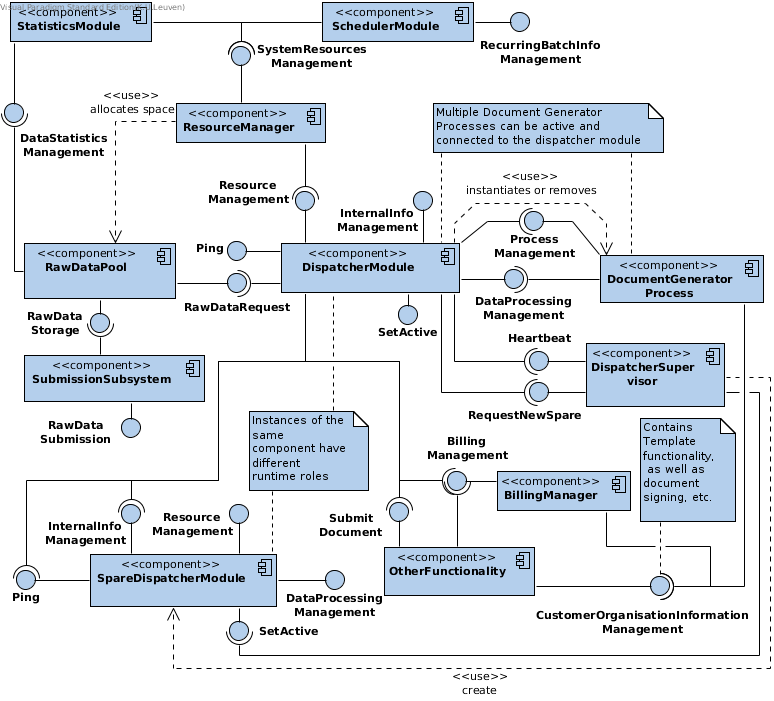
\includegraphics[width=\textwidth]{comp_diag_1.png}
    %\missingfigure[figwidth=0.8\textwidth]{Component-and-connector diagram}
    \caption{Component-and-connector diagram of this decomposition.}\label{fig:it1-cc_main}
\end{figure}

\paragraph{Behaviour}
Figure \ref{fig:it1-seq_aspect1} illustrates the standard flow of document generation in the system. This flow is initiated by the \texttt{GeneratorProcesses} themselves. When new a new Raw Data Entry is requested and none is found, \texttt{GeneratorProcesses} go into standby. When the \texttt{DispatcherModule} is notified of new data being available, it can reactivate the \texttt{GeneratorProcesses}.

\begin{figure}[!htp]
    \centering
    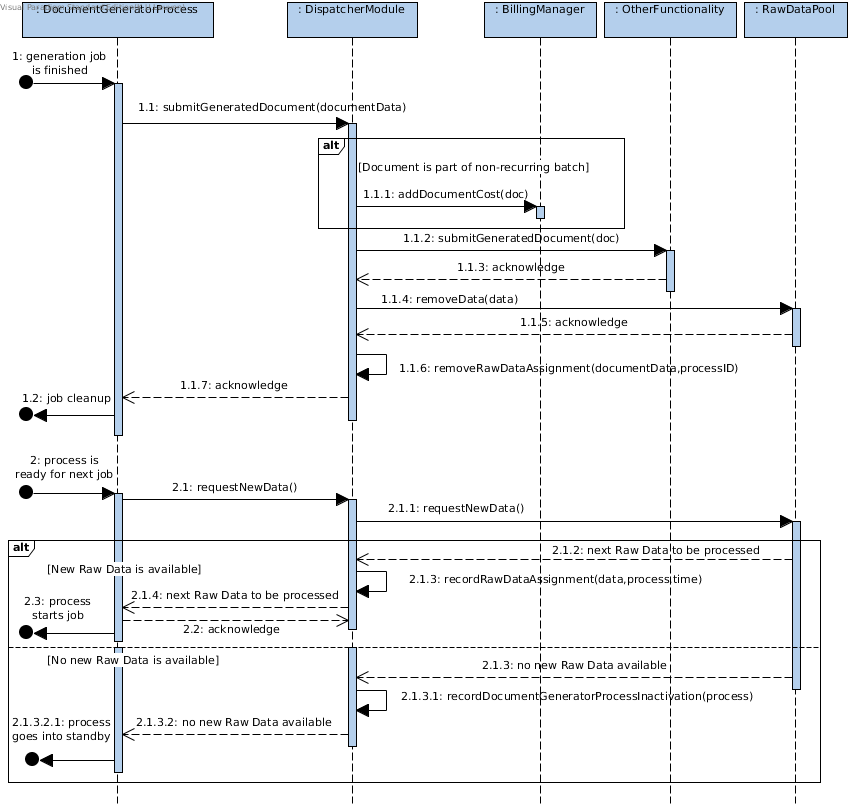
\includegraphics[width=\textwidth]{seq_diag_1_-_doc_gen.png}
    %\missingfigure[figwidth=0.8\textwidth]{Sequence diagram}
    \caption{Sequence diagram illustrating the flow of document generation.}\label{fig:it1-seq_aspect1}
\end{figure}

\paragraph{Deployment}
Figure \ref{fig:it1-depl_main} shows the mapping of architectural components on physical nodes.
The main entry point and accompanying storage components of the system are gathered on the \texttt{RawDataHandlingNode}, since these work together closely and depend on eachother. Also, they are a cohesive part of the system regarding behaviour. The \texttt{DispatcherSupervisor} and both \texttt{DispatcherModule}s are key components in the system, being the central focus of generation behaviour. They each have their own node, being essential parts, so simultaneous failure is less likely. The \texttt{DocumentGeneratorProcesses} are mapped to their own dedicated nodes because they are work processes and specialised powerful nodes can be provided to them. They can be distributed along multiple of these nodes so that when a lot of work is done, failure of one work node doesn't bring the system to a halt. The remaining functionality of the system, most of which is used later than the behaviour specified by the selected drivers, is mapped to an OtherFunctionalityNode, which is to be decomposed later.

\begin{figure}[!htp]
    \centering
    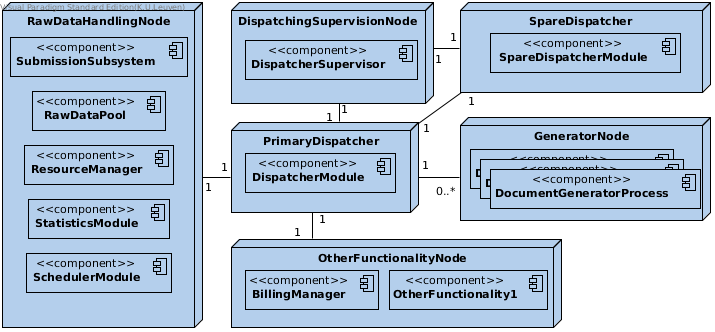
\includegraphics[width=0.8\textwidth]{depl_diag_1.png}
    %\missingfigure[figwidth=0.8\textwidth]{Deployment diagram}
    \caption{Deployment diagram of this decomposition.}\label{fig:it1-depl_main}
\end{figure}

\subsubsection{Interfaces for child modules}
\subsubsection*{DispatcherModule}
\begin{itemize}
    \item DataProcessingManagement
    \begin{itemize}
        \item \texttt{RawDataEntry requestNewData()}
        \begin{itemize}
            \item Effect: Supply a new Raw Data Entry. May be an empty entry if no Raw Data Entry is available.
            \item Exceptions: None
        \end{itemize}

        \item \texttt{void submitGeneratedDocument(DocumentData generated)} throws InvalidDocumentDataException
        \begin{itemize}
            \item Effect: Accept a generated document so that it may be delivered and the Customer Organization billed if appropriate.
            \item Exceptions:
            \begin{itemize}
            	\item InvalidDocumentDataException: The DocumentData argument is badly structured
            \end{itemize}
        \end{itemize}

        \item \texttt{void signalDocumentGenerationFailure(GenerationErrorReport report)}
        \begin{itemize}
        	\item Effect: Passes the given GenerationErrorReport on through appropriate channels
        	\item Exceptions: None
        \end{itemize}

        \item \texttt{void renewLease(RawDataEntryID id)} throws LeaseExpiredException
        \begin{itemize}
            \item Effect: Renew the lease on the Raw Data Entry with given ID.
            \item Exceptions:
            \begin{itemize}
                \item LeaseExpiredException: Thrown when the lease has already expired, or the \texttt{DocumentGenerationProcess} has reached the maximum amount of lease renewals.
            \end{itemize}
        \end{itemize}
    \end{itemize}
	\item Ping
	\begin{itemize}
		\item \texttt{Echo ping()}
		\begin{itemize}
			\item Effect: Returns an Echo to reassure the caller that the callee is still available.
			\item Exceptions: None
		\end{itemize}
	\end{itemize}
\end{itemize}

\begin{itemize}
	\item ResourceManagement
	\begin{itemize}
		\item \texttt{void notify(ResourceGuidelineReport report)}
		\begin{itemize}
			\item Effect: Supply information that is relevant to how many \texttt{DocumentGeneratorProcess}es the \texttt{DispatcherModule} should maintain. The \texttt{DispatcherModule} returns immediately and thereafter takes appropriate actions (e.g. instantiate new \texttt{DocumentGeneratorProcess}es).
			\item Exceptions: None
		\end{itemize}
	\end{itemize}
\end{itemize}

%\todo{Verification of data when spare becomes active}
\begin{itemize}
	\item InternalInfoManagement
	\begin{itemize}
		\item \texttt{void recordNewDocumentGeneratorProcess(DocumentGeneratorProcessID id)}
		\begin{itemize}
			\item Effect: Records the identifier of a new \texttt{DocumentGeneratorProcess}. No effect if the identifier has been supplied previously.
			\item Exceptions: None
		\end{itemize}

		\item \texttt{void recordDocumentGeneratorProcessRemoval(DocumentGeneratorProcessID id)}
		\begin{itemize}
			\item Effect: Records that the \texttt{DocumentGeneratorProcess} with the specified identifier has been removed from the system. No effect if the identifier was not supplied earlier through \texttt{recordNewDocumentGeneratorProcess(DocumentGeneratorProcessID)}.
			\item Exceptions: None
		\end{itemize}

		\item \texttt{void recordRawDataAssignment(RawDataEntry entry, DocumentGeneratorProcessID id,Time t)}
		\begin{itemize}
			\item Effect: Records that the specified Raw Data Entry has been assigned to the specified \texttt{DocumentGeneratorProcess} on timepoint \texttt{t}. If that pair of Raw Data Entry and \texttt{DocumentGeneratorProcess} has already been recorded with a certain time \texttt{t2}, the new time overwrites the old.
			\item Exceptions: None
		\end{itemize}

		\item \texttt{void removeRawDataAssignment(DocumentData generated, DocumentGeneratorProcessID id)}
		\begin{itemize}
			\item Effect: Removes the assignment of the Raw Data Entry in the specified DocumentData to the specified \texttt{DocumentGeneratorProcess}. No effect if that pair is not recorded.
			\item Exceptions: None
		\end{itemize}

		\item \texttt{void recordGeneratedDocument(DocumentData generated, DocumentGeneratorProcessID id)}
		\begin{itemize}
			\item Effect: Stores the supplied generated document in secondary storage, along with an ID for the \texttt{GeneratorProcess}, to be able to deliver an acknowledgement.
			\item Exceptions: None
		\end{itemize}

		\item \texttt{void removeGeneratedDocument(DocumentDataID id)} throws DocumentNotFoundException
		\begin{itemize}
			\item Effect: Deletes the corresponding DocumentData from secondary storage.
			\item Exceptions:
			\begin{itemize}
				\item DocumentNotFoundException: No corresponding DocumentData exists in storage.
			\end{itemize}
		\end{itemize}

		\item \texttt{void recordDocumentGeneratorProcessInactivation(DocumentGeneratorProcessID id)}
		\begin{itemize}
			\item Effect: Marks the corresponding \texttt{GeneratorProcess} as inactive due to no new Raw Data being available.
			\item Exceptions: None
		\end{itemize}
	\end{itemize}
\end{itemize}

\begin{itemize}
	\item SetActive
	\begin{itemize}
		\item \texttt{void activate()} throws AlreadyActiveException
		\begin{itemize}
			\item Effect:
			\begin{itemize}
				\item Looks up and assumes control of all \texttt{DocumentGeneratorProcess}es it has an identifier of.
				\item Verifies the correctness of its internal state by contacting the \texttt{RawDataPool} (to verify which Raw Data Entries have been marked as work in progress), \texttt{DocumentGeneratorProcess}es (to verify assignments of Raw Data Entries to \texttt{Processes}) and \texttt{OtherFunctionality1} (to verify which generated documents it has in storage have already been delivered.
				\item Requests a new \texttt{SpareDispatcherModule} from the \texttt{DispatcherSupervisor}
				\item Copies its state to the new spare
				\item Returns and resumes normal operation
			\end{itemize}
			\item Exceptions:
			\begin{itemize}
				\item AlreadyActiveException: This \texttt{DispatcherModule} is the active \texttt{DispatcherModule}
			\end{itemize}
		\end{itemize}
	\end{itemize}
\end{itemize}

\subsubsection*{DocumentGeneratorProcess}
\begin{itemize}
	\item ProcessManagement
	\begin{itemize}
		\item \texttt{ProcessStatusReport getStatusReport(RawDataEntryID id)}
		\begin{itemize}
			\item Effect: Indicates through the returned object whether it is working on the specified Raw Data Entry and if it has finished or not
			\item Exceptions: None
		\end{itemize}

		\item \texttt{Echo ping()}
		\begin{itemize}
			\item Effect: Returns an Echo to reassure the caller that the callee is still available.
			\item Exceptions: None
		\end{itemize}

		\item \texttt{void assignRawData(RawDataEntry entry)} throws NotIdleException
		\begin{itemize}
			\item Effect: Assigns the specified RawDataEntry to this \texttt{DocumentGeneratorProcess}
			\item Exceptions:
			\begin{itemize}
				\item NotIdleException: This \texttt{DocumentGeneratorProcess} is already working on another RawDataEntry.
			\end{itemize}
		\end{itemize}

		\item \texttt{DocumentData getGeneratedDocument()} throws NoDocumentDataAvailableException
		\begin{itemize}
			\item Effect: Supplies the document generated from its assigned Raw Data Entry
			\item Exceptions:
			\begin{itemize}
				\item NoDocumentDataAvailableException: Document generation has not yet been finished or no RawDataEntry has been assigned.
			\end{itemize}
		\end{itemize}
	\end{itemize}
\end{itemize}

\subsubsection*{RawDataPool}
\begin{itemize}
	\item GetNextRawData
	\begin{itemize}
		\item \texttt{RawDataEntry requestNewData()}
		\begin{itemize}
			\item Effect: Supplies the next RawDataEntry that should be processed. If no Entry is available, an empty Entry is returned.
			\item Exceptions: None
		\end{itemize}

		\item \texttt{PoolDataReport getDataReport()}
		\begin{itemize}
			\item Effect: Supplies information about which RawDataEntry entries have been marked as work in progress.
			\item Exceptions: None
		\end{itemize}

		\item \texttt{void removeData(RawDataEntryID id)} throws NoSuchRawDataEntryException
		\begin{itemize}
			\item Effect: Removes the corresponding RawDataEntry from the pool.
			\item Exceptions:
			\begin{itemize}
				\item NoSuchRawDataEntryException: There is no corresponding RawDataEntry.
			\end{itemize}
		\end{itemize}
	\end{itemize}
\end{itemize}

\begin{itemize}
	\item SubmitDataForProcessing
	\begin{itemize}
		\item \texttt{void submitRawDataBatch(RawDataBatch data)}
		\begin{itemize}
			\item Effect: Adds the RawData in the specified RawDataBatch to the pool. A unique identifier is generated for each RawData and the resulting RawDataEntry entries are scheduled according to the scheduling policy.
			\item Exceptions: None
		\end{itemize}
	\end{itemize}
\end{itemize}

\subsubsection*{DispatcherSupervisor}
\begin{itemize}
	\item Heartbeat
	\begin{itemize}
		\item \texttt{void supplyHeartbeat()}
		\begin{itemize}
			\item Effect: Records a heartbeat from the supervised component.
			\item Exceptions: None
		\end{itemize}
	\end{itemize}
\end{itemize}

\begin{itemize}
	\item Failure Management
	\begin{itemize}
		\item \texttt{DispatcherID requestNewSpareDispatcher()}
		\begin{itemize}
			\item Effect: Initialises a new \texttt{SpareDispatcherModule} and generates an ID for it such that callee can find the new spare.
			\item Exceptions: None
		\end{itemize}

	    \item \texttt{void signalDocumentGenerationFailure(GenerationErrorReport report)}
	    \begin{itemize}
		    \item Effect: Passes on the given GenerationErrorReport through appropriate channels.
		    \item Exceptions: None
	    \end{itemize}

	    \item \texttt{void signalDocumentGeneratorProcessFailure(GeneratorProcessFailureReport report)}
	    \begin{itemize}
		    \item Effect: Passes on the given GeneratorProcessFailureReport through appropriate channels.
		    \item Exceptions: None
	    \end{itemize}
    \end{itemize}
\end{itemize}

\subsubsection*{StatisticsModule}
\begin{itemize}
	\item DataStatisticsManagement
	\begin{itemize}
		\item \texttt{void deliver(StatisticsReport report)}
		\begin{itemize}
			\item Effect: Integrates the information supplied by the given report into its own information (e.g. mean pool capacity during a certain period in a certain month).
			\item Exceptions: None
		\end{itemize}
	\end{itemize}
\end{itemize}

\subsubsection*{SchedulerModule}
\begin{itemize}
	\item RecurringBatchInfoManagement
	\begin{itemize}
		\item \texttt{void recordRecurringBatch(Date date, int maxAmount)}
		\begin{itemize}
			\item Effect: Records that a batch with the specified maximal amount is expected at the specified date.
			\item Exceptions: None
		\end{itemize}

		\item \texttt{void deleteRecurringBatch(Date date, int maxAmount)}
		\begin{itemize}
			\item Effect: Records that a batch on the specified date with the specified maximal amount will no longer occur.
			\item Exceptions: None
		\end{itemize}
	\end{itemize}
\end{itemize}

\subsubsection*{ResourceManager}
\begin{itemize}
    \item SystemResourceManagement
    \begin{itemize}
        \item \texttt{void recommendPoolCapacity(long poolSize)}
        \begin{itemize}
            \item Effect: Recommends the ResourceManager to scale the \texttt{RawDataPool} to given size.
            \item Exceptions: None
        \end{itemize}

        \item \texttt{void recommendProcessingJobsAmount(int amount)}
        \begin{itemize}
            \item Effect: Recommends the ResourceManager to regulate the amount of \texttt{DocumentGeneratorProcesses} to given amount.
            \item Exceptions: None
         \end{itemize}
    \end{itemize}
\end{itemize}

\subsubsection*{SubmissionSubsystem}
\begin{itemize}
	\item RawDataSubmission
	\begin{itemize}
		\item \texttt{void submitRawDataBatch(RawDataBatch batch)}
		\begin{itemize}
			\item Effect: Submits the given RawDataBatch for processing.
			\item Exceptions: None
		\end{itemize}
	\end{itemize}
\end{itemize}

\subsubsection*{BillingManager}
\begin{itemize}
	\item BillingManagement
	\begin{itemize}
		\item \texttt{void billCustomer(RawDataEntry entry)}
		\begin{itemize}
			\item Effect: Extracts the required information to bill the Customer Organization for generation of the document from the RawDataEntry (e.g. document type, priority) on the one hand and from Customer Organization information stored elsewhere in the system on the other hand and records a new billing for the Customer Organization.
			\item Exceptions: None
		\end{itemize}
	\end{itemize}
\end{itemize}

\subsubsection*{OtherFunctionality1}
\begin{itemize}
	\item SubmitDocument
	\begin{itemize}
		\item \texttt{void submitDocument(DocumentData data)}
		\begin{itemize}
			\item Effect: Initiates the submission process for the specified generated document
			\item Exceptions: None
		\end{itemize}

		\item \texttt{boolean isDocumentSubmitted(DocumentDataID data)}
		\begin{itemize}
			\item Effect: Indicates whether the generated document corresponding to the given DocumentDataID has already been delivered.
			\item Exceptions: None
		\end{itemize}
	\end{itemize}
	\item CustomerOrganisationInformationManagement
	\begin{itemize}
	    \item \texttt{Template getTemplateOfType(DocumentType type, OrganisationID id)} throws InvalidIDException, UnsupportedTypeException
	    \begin{itemize}
	        \item Effect: Look up and returns the Template, registered by \texttt{Customer Organisation} for given Document Type.
	        \item Exceptions:
	        \begin{itemize}
	            \item InvalidIDException: When an ID is supplied that does not match any \texttt{Customer Organisation}.
	            \item UnsupportedTypeException: When \texttt{Customer Organisation} with given ID is not registered for given Document Type (relevant for \emph{M1: New type of document: bank statements}, where adoption of a new Document Type is not mandatory for a \texttt{Customer Organisation}, while in the base case it may be).
	        \end{itemize}
	    \end{itemize}
	    \item \texttt{DocumentData signDocument(DocumentData data)} throws AlreadySignedException
	    \begin{itemize}
	        \item Effect: Signs the Document in the Document Data with the signing key of the Customer Organisation, which can be looked up with the ID found in the Document Data. Afterwards, returns the Document Data, with as only alteration the signing of the Document inside.
	    \end{itemize}
	\end{itemize}

	\item AdminNotificationDelivery
	\begin{itemize}
		\item \texttt{void deliverAdminNotification(AdminNotification notification)}
		\begin{itemize}
			\item Effect: Delivers the specified AdminNotification to the intended recipient
			\item Exceptions: None
		\end{itemize}
	\end{itemize}
\end{itemize}

\subsubsection*{AdminNotificationHandler}
\begin{itemize}
	\item AdminNotificationManagement
	\begin{itemize}
		\item \texttt{void signalDocumentGenerationFailure(GenerationErrorReport report)}
		\begin{itemize}
			\item Effect: Passes the specified GenerationErrorReport on to the appropriate Customer Organization Administrator
			\item Exceptions: None
		\end{itemize}
	\end{itemize}

	\begin{itemize}
		\item \texttt{void signalDocumentGeneratorProcessFailure(GeneratorProcessFailureReport report)}
		\begin{itemize}
			\item Effect: Passes the specified GeneratorProcessFailureReport on to the eDocs administrators
			\item Exceptions: None
		\end{itemize}
	\end{itemize}

	\begin{itemize}
		\item \texttt{void signalDispatcherModuleFailure(DispatcherModuleFailureReport report)}
		\begin{itemize}
			\item Effect: Passes the specified DispatcherModuleFailureReport on to the eDocs administrators
			\item Exceptions: None
		\end{itemize}
	\end{itemize}
\end{itemize}

\subsubsection{Data type definitions}
This section provides an overview of all complex data types used in the interfaces.

\paragraph{RawData} Contains the data from which a single document can be generated and the meta-data relevant to that document (e.g. recipient information and Customer Organization that submitted the data).

\paragraph{RawDataBatch} Contains several RawData instances

\paragraph{RawDataEntryID} Allows unique identification of a single RawDataEntry instance.

\paragraph{RawDataEntry} The combination of a RawData instance and its corresponding RawDataEntryID.

\paragraph{DocumentData} Represents a generated document and the raw data from which it was generated.

\paragraph{DocumentType} Represents a certain document type.

\paragraph{Template} Provides a skeleton for a document of a certain document type. It has fields that can be filled out with raw data.

\paragraph{DocumentDataID} Allows unique identification of a single DocumentData instance.

\paragraph{Echo} A message used as response to a ping request.

\paragraph{ResourceGuidelineReport} Encapsulates directives from the \texttt{ResourceManager} or the \texttt{RawDataPool} regarding the desired amount of active \texttt{DocumentGeneratorProcess}es. Those guidelines are due to either imminent recurring batches, past resource usage patterns or high \texttt{RawDataPool} capacity usage.

\paragraph{DocumentGeneratorProcessID} Allows look-up of the corresponding unique \texttt{DocumentGeneratorProcess}.

\paragraph{ProcessStatusReport} Encapsulates information regarding a \texttt{DocumentGeneratorProcess} such as which, if any, RawDataEntry it is working on and whether it has finished generating the document or not.

\paragraph{PoolDataReport} Reports which RawDataEntry entries in the \texttt{RawDataPool} have been marked as work in progress.

\paragraph{StatisticsReport} Encapsulates information about resource usage (e.g. currently used \texttt{RawDataPool} capacity at a certain time)

\paragraph{OrganisationID} Allows unique identification of a single Customer Organisation

\paragraph{DispatcherID} Allows look-up of a single unique \texttt{DispatcherModule} instance

\paragraph{GenerationErrorReport} Contains the RawDataEntryID for which generation failed and information as to why it failed

\paragraph{GeneratorProcessFailureReport} Contains the DocumentGeneratorProcessID of the \texttt{DocumentGeneratorProcess} that failed and any specifics known about the failure

\paragraph{DispatcherModuleFailureReport} Contains the DispatcherID of the \texttt{DispatcherModule} that failed and any specifics known about the failure

\paragraph{AdminNotification} Contains one of several possible report types that can be addressed to either eDocs Administrators or Customer Administrators (e.g. GenerationErrorReport, GeneratorProcessFailureReport, DispatcherModuleFailureReport)

\subsubsection{Verify and refine}
This section describes per component which (parts of) the remaining requirements it is responsible for. If requirements are split, a letter is added to its name (e.g. Av1a) to indicate that the component will only satisfy a part of the original requirement. If requirements are split, it will also be indicated what part of the original requirement each new requirement contains. If new derived requirements are introduced they will receive a new identifier and are marked as a new requirement.

\paragraph{OtherFunctionality1}
\begin{itemize}
    \item \emph{UC1}: Log in
    \item \emph{UC2}: Log out
    \item \emph{UC6}: Deliver document via e-mail
    \item \emph{UC7}: Notify of e-mail delivery failure
    \item \emph{UC8}: Deliver document via postal mail
    \item \emph{UC9}: Deliver invoice via Zoomit
    \item \emph{UC10}: Confirm document delivery (Zoomit)
    \item \emph{UC11}: Deliver document via personal document store
    \item \emph{UC12}: Consult personal document store
    \item \emph{UC13}: Search documents in personal document store
    \item \emph{UC14}: Consult document in personal document store
    \item \emph{UC15}: Download document via unique link
    \item \emph{UC16}: Register to personal document store
    \item \emph{UC17}: Unregister from personal document store
    \item \emph{UC18}: Register customer organization
    \item \emph{UC19}: Unregister customer organization
    \item \emph{UC20}: Update document template
    \item \emph{UC21a}: Consult status of all document processing jobs\\
    Handling the (visual) interfacing with the user. Determining the finished jobs.
    \item \emph{UC22a}: Notify customer administrator
    Notifying the customer administrator of delivery failure
    \item \emph{Av2}: Personal document storage failure
    \item \emph{Av3}: Zoomit failure
    \item \emph{P2}: Document lookups
    \item \emph{P3a}: Status overview for customer administrators\\
    Handling the flow of this requirement and the overal processing of the status reports in a timely fashion.
    \item \emph{M1a}: New type of document: bank statements\\
    The delivery and template handling for the new document.
    \item \emph{M2}: Multiple print \& postal services
    \item \emph{M3}: Dynamic selection of the cheapest of print \& postal services
\end{itemize}

\paragraph{SubmissionSubsystem}
\begin{itemize}
    \item \emph{UC3}: Initiate document processing
    \item \emph{M1b}: New type of document: bank statements\\
    Being able to receive and verify the integrity of Raw Data for the new type of document.
\end{itemize}

\paragraph{RawDataPool}
\begin{itemize}
    \item \emph{UC21b}: Consult status of all document processing jobs\\
    Determining the unfinished and currently processing jobs.
    \item \emph{P3b}: Status overview for customer administrators\\
    Calculating and delivering information about all unfinished and currently processing jobs for a certain \texttt{Customer Organisation} in a timely fashion.
\end{itemize}

\paragraph{DocumentGenerationProcess}
\begin{itemize}
    \item \emph{M1c}: New type of document: bank statements\\
    Being able to generate documents of the new type with the accompanying new template.
\end{itemize}

\subsection{Decomposition 2: OtherFunctionality1 (Av2, UC11, UC12, UC13, UC14)}
\subsubsection{Module to decompose}
In this run we decompose \texttt{OtherFunctionality1}. This component is an aggregate of leftover behaviour in the previous run.

\subsubsection{Selected architectural drivers}
The non-functional drivers for this decomposition are:

\begin{itemize}
    \item \emph{Av2}: Personal document storage failure
    \item \emph{P2}: Document Lookups
\end{itemize}

The related functional drivers are:

\begin{itemize}
    \item \emph{UC11}: Deliver document via personal document store
    \item \emph{UC12}: Consult personal document store
    \item \emph{UC13}: Search documents in personal document store
    \item \emph{UC14}: Consult document in personal document store
\end{itemize}

\paragraph{Rationale}
These drivers are the main drivers concerned with normal usage of the personal document store. No components regarding authentication or registering are considered. These drivers are also either High or Medium priority, making them a good choice.

\subsubsection{Architectural design}

\paragraph{Storage of generated documents}
When the \texttt{DispatcherModule} (cf. decomposition 1) submits a document, it first arrives at the \texttt{GeneratedDocumentHandler}. It is here that it is decided what exactly to do with the document. It is offered to the \texttt{ReplicationManager} (see paragraph ``Prevention and detection of document storage (\emph{Av2})'') regardless, but other actions may also be appropriate based on the raw data supplied along with the document, such as generating a download link or submitting the document to a certain delivery subsystem, e.g. the postal delivery subsystem.

\paragraph{Prevention and detection of document storage failure (\emph{Av2})}
\emph{Av2} specifies that the personal document storage should have a guaranteed minimal up-time. We propose a \texttt{DocumentDB}, which stores all generated documents, and the \texttt{PersonalDocumentDatabase}, which stores references (or documents themselves, see ``\texttt{PersonalDocumentDatabase}'' under ``Instantiation and allocation of functionality''),  to the documents together with an identifier of the registered recipient to which those documents are addressed (see paragraph ``Splitting up the document database and personal document database'' for the rationale as to why these two are split up). Part of the solution to the prevention problem is to have passive replication of both the document database and the personal document database. We therefore propose a \texttt{ReplicationManager} that manages both the replicas of the \texttt{DocumentDB} and \texttt{PersonalDocumentDatabase}. The \texttt{ReplicationManager} manages both kinds of databases since the contents of both are tied closely together, therefore having separate replication managers for both would entail unnecessary overhead. The replicas of the respective databases are called the \texttt{SecondaryDB} and \texttt{SecondaryPersonalDocumentDatabase}. When a generated document arrives at the \texttt{ReplicationManager}, it stores the document in the \texttt{DocumentDB} and, if appropriate, also stores a reference to the document together with an identifier of the recipient in the \texttt{PersonalDocumentDatabase}. As we have opted for passive replication, both databases shall implement an interface through which their respective primaries can synchronise with their secondaries. This synchronisation will happen every ten minutes. It is possible that the primary crashes before it has synchronised any new data. To solve this, we introduce the \texttt{DocumentSubmissionCache}, which stores 3 hours worth of updates for both databases. When a secondary of either type is activated, the relevant updates in the \texttt{DocumentSubmissionCache} are flushed to the new primary. The fact that some of those updates may already have been present poses no problem as writes are idempotent. In order to detect failure of the current primary, both databases also implement a ping interface so that the \texttt{ReplicationManager} can detect failure in a timely manner and send out a notification to the eDocs administrators.

\paragraph{Handling failure of the personal document storage (\emph{Av2})}
\emph{Av2} specifies that documents to be delivered via the personal document store must be temporarily stored elsewhere if the personal document storage fails. In our set-up, the \texttt{DocumentSubmissionCache} is also responsible for caching whichever type of records a database stores if it fails. When normal operation is resumed, the \texttt{ReplicationManager} must then write all records of the correct type stored in the \texttt{DocumentSubmissionCache} into the database. At least three hours of corresponding entries must be stored until the failure is resolved. Therefore, when the \texttt{PersonalDocumentDatabase} and all replicas fail, all personal document records that arrive in the meantime are written to the \texttt{DocumentSubmissionCache}, which are then written to the \texttt{PersonalDocumentDatabase} when it resumes operation.

\paragraph{Degraded mode upon failure of personal document store (\emph{Av2})}
\emph{Av2} requires that a maximally functional interface is presented to the user when they attempt to access the personal document store after it has failed. In order to realise this, we add a module that queries the \texttt{PersonalDocumentDatabase} on the user's behalf, the \texttt{PersonalDocumentLookupModule}. When a request of the \texttt{PersonalDocumentLookupModule} times out, it pings the \texttt{PersonalDocumentDatabase}. If no response is received within five seconds, it is determined that the \texttt{PersonalDocumentDatabase} has failed. The request fails and this is indicated to the user. The \texttt{PersonalDocumentLookupModule} keeps pinging the \texttt{PersonalDocumentDatabase} every ten seconds. Upon reception of an echo, normal operation is resumed. While the \texttt{PersonalDocumentLookupModule} is still pinging the \texttt{PersonalDocumentDatabase}, any further requests result in an indication that the personal document storage is currently unavailable.

\paragraph{Detecting failure of the \texttt{GeneratedDocumentHandler}}
The \texttt{GeneratedDocumentHandler} is a rather sensitive point in the system, as all generated documents must pass through here. Therefore, we introduce the \texttt{GenDocHandlerListener} that monitors the heartbeat of the \texttt{GeneratedDocumentHandler} and notifies an eDocs administrator through the \texttt{AdminNotificationHandler} upon determination of failure.

\paragraph{Maintaining download links for documents}
Any document sent to an unregistered recipient is associated with a download link if receipt tracking has been activated. In order to manage this, we propose the \texttt{DownloadDocumentLookupModule}. When the \texttt{GeneratedDocumentHandler} submits a document to the \texttt{DownloadDocumentLookupModule}, it generates a unique link. This link is then stored together with the time at which it was generated. When download of a document is initiated, the link is submitted to the \texttt{DownloadDocumentLookupModule} inside a download token, which then queries the \texttt{DocumentDB}. If the link has expired in the meantime, this is indicated to the user. The \texttt{DownloadDocumentLookupModule} periodically checks if any of its links have expired. If it detects expired links, the appropriate Customer Administrator and recipient are notified.

\paragraph{Lookup of documents in the personal document storage}
Support must be provided for consulting a user's personal document store as a whole, consulting a specific document or searching through the personal document store. We therefore make the \texttt{PersonalDocumentLookupModule} capable of issuing diverse types of queries. It can request summaries of all of a user's documents, request a full document matching a certain document reference, or issue a query ((partial) name of the sender, type of document, date range, etc.) the documents of interest must match, which also produces summaries of all matching documents. In all of these requests, the user's identifier is implicitly included as a parameter.

\paragraph{Load balancing (\emph{P2})}
\emph{P2} specifies that requests for documents in the personal document store or requests for downloads must be throttled under certain circumstances. In order to realise this, we propose the \texttt{LookupLoadBalancer}. Both the \texttt{DownloadDocumentLookupModule} and the \texttt{PersonalDocumentLookupModule} must receive permission from the \texttt{LookupLoadBalancer} before issuing an individual lookup. Also, when either module has finished executing a lookup, they must report to the \texttt{LookupLoadBalancer} which kind of lookup it was and how long they took executing it. This way, the \texttt{LookupLoadBalancer} can determine when there is a high load on the system and delay giving permission for execution of lookups where appropriate. Other components in the system can also keep the \texttt{LookupLoadBalancer} aware of currently existing processing capacity so that it can keep this information in mind when making decisions.

\subsubsection*{Alternatives considered}
\paragraph{Splitting up the document database and personal document database}
Several options exist as to how to implement the personal document store. One of these is to simply keep all documents in document storage. If this is done, then there is a virtual personal document store for each user. This is deemed undesirable, as the personal document store of a certain user must then be computed every time a request comes in. The overhead introduced by this can be substantial when a lot of documents have been stored and the personal document store of a user is large. All other options consist of somehow redundantly storing all documents that belong to a personal document store. The obvious solution would be to store all those documents in the document storage and also in a dedicated personal document storage. This proposal was also rejected, as the document storage already has passive replication in place and this solution would introduce an unacceptable level of redundancy. The solution currently in place (i.e. storing references to documents instead of the full documents) was deemed to be sufficiently low-impact in terms of storage while still offering acceptable performance for the personal document store.

\paragraph{Passive replication vs active replication for document storage}
\emph{Av2} specifies that documents must temporarily be stored elsewhere upon failure. The affected documents are then processed when normal operation is resumed. Passive replication is a natural fit for this requirement since it involves synchronisation, both during normal operation and after failure of the primary. Using active replication for this purpose would still require some sort of cache in order to meet this requirement, which does not agree with the principle of active replication.

\paragraph{Ping/echo versus heartbeat for document storage}
The \texttt{ReplicationManager} must detect when the primary fails. Acknowledgements are implicit each time the primary indicates it has successfully executed a write, therefore using a heartbeat would be of limited use. It is only when the primary fails to acknowledge a write that the \texttt{ReplicationManager} must explicitly ascertain whether the primary is still alive, and using ping/echo is perfect for this purpose.

\subsubsection{Instantiation and allocation of functionality}
\paragraph{Decomposition}
Figure \ref{fig:it2-cc_main} shows the components resulting from the decomposition in this run. The same clarification concerning the \texttt{DispatcherModule} and \texttt{SpareDispatcherModule} has to be made for both the \texttt{DocumentDB} and \texttt{SecondaryDocumentDB} and the \texttt{PersonalDocumentDatabase} and \texttt{SecondaryPersonalDocumentDatabase} respectively. These components are pairwise instantiations of the same type of component with different runtime responsibilities. This is noticable from the fact they have the same interfaces but different ones are being used on either. Additional notes are added to the diagram where deemed necessary.

\subparagraph{GeneratedDocumentHandler}
This component is the entry point for the delivery subsystem from the generation subsystem. It accepts generated documents and determines where and how these should be delivered. It submits these documents to the \texttt{ReplicationManager} to place it in the general \texttt{DocumentDB}, along with instructions whether or not it should also place these in the \texttt{PersonalDocumentDatabase}. It should bill Customer Organisations for the delivery of non-recurring batch documents, after determining this property for a received document. It signals the \texttt{GenDocHandlerListener} periodically to convey that it is still alive (This is a consideration made because of the fact that it is a Single Point of Failure in the system). Also responsible for composing a message to the user that a new document is available, when necessary, and delivering this to the \texttt{RecipientNotificationModule}. When necessary, instructs the \texttt{DownloadDocumentLookupModule} to record a deadline for a document download for a certain client and document.

\subparagraph{GenDocHandlerListener}
Listens to the heartbeat signal of the \texttt{GeneratedDocumentHandler} to ascertain it remaining functional. When the \texttt{GeneratedDocumentHandler} fails to signal the fact that it still functions, it is considered failed, and the \texttt{GenDocHandlerListener} notifies the eDocs Administrator of this fact through the \texttt{AdminNotificationHandler}.

\subparagraph{ReplicationManager}
Handles the passive replication for both the \texttt{DocumentDB} and the \texttt{PersonalDocumentDatabase}. It is responsible for both since they are tied together closely. When either fails and the \texttt{ReplicationManager} does not receive an answer for a while, the affected component is pinged, and when it does not answer, the \texttt{ReplicationManager} notifies the eDocs Administrator of this fact through the \texttt{AdminNotificationHandler}. When a document is received from the \texttt{GeneratedDocumentHandler}, it submits this to the \texttt{DocumentDB}, and if so instructed also in the \texttt{PersonalDocumentDatabase}. It also places the document in the \texttt{DocumentSubmissionCache}, indicating whether the document should be stored in the \texttt{DocumentDB} and/or the \texttt{PersonalDocumentDatabase}. It removes this document from the cache when it has received a confirmation that the document has been replicated onto all secondary databases it should belong to.

\subparagraph{DocumentSubmissionCache}
Accepts documents that should be temporarily stored before they are replicated in the databases. Allows for at least 3 hours of received document storage. Removes the documents from its storage when signaled to do so by the \texttt{ReplicationManager}.

\subparagraph{DocumentDB}
General database for all generated documents. Accepts documents from the \texttt{ReplicationManager} for storage. It should synchronize with the \texttt{SecondaryDocumentDB} periodically to keep their states consistent, and signals the \texttt{ReplicationManager} which documents have been succesfully replicated in both \texttt{DocumentDB}s. It should provide the \texttt{PersonalDocumentDatabase} with a requested document when so instructed by it. It should respond to pings by the \texttt{ReplicationManager}.

\subparagraph{SecondaryDocumentDB}
Accepts synchronisation requests from the \texttt{DocumentDB}, replicating any documents from the \texttt{DocumentDB} it does not yet contain, and then answer that it has succesfully done so.

\subparagraph{PersonalDocumentDatabase}
Specialised database for the personal document store service. Accepts documents from the \texttt{ReplicationManager} for storage. Keeps a set amount of documents in storage per Registered Recipient. When a new document for a user arrives and the maximum amount of documents for this user in the \texttt{PersonalDocumentDatabase} is reached, the oldest document is replaced by a reference to it in the \texttt{DocumentDB}. It should synchronize with the \texttt{SecondaryPersonalDocumentDatabase} periodically to keep their states consistent, and signals the \texttt{ReplicationManager} which documents or references have been succesfully replicated in both \texttt{PersonalDocumentDatabase}s. It should provide the \texttt{PersonalDocumentLookupModule} with a requested document when so instructed by it, and if it only has a corresponding reference, queries the \texttt{DocumentDB} for it. It should respond to pings by the \texttt{ReplicationManager}.

\subparagraph{SecondaryPersonalDocumentDatabase}
Accepts synchronisation requests from the \texttt{PersonalDocumentDatabase}, replicating any documents or references from the \texttt{PersonalDocumentDatabase} it does not yet contain, and then answer that it has succesfully done so.

\subparagraph{PersonalDocumentLookupModule}
Accepts requests to serve documents out of the \texttt{PersonalDocumentDatabase}, querying the \texttt{PersonalDocumentDatabase} for them and returning them. When the \texttt{PersonalDocumentDatabase} does not answer, it is pinged, and when it fails to respond, the \texttt{PersonalDocumentLookupModule} returns the answer that the personal document stores are currently unavailable. Before looking up a document, it should ask the \texttt{LookupLoadBalancer} first if it is allowed to do so. After having looked up a document, it should also notify the \texttt{LookupLoadBalancer} of this, along with the effective delay it encountered.

\subparagraph{DownloadDocumentLookupModule}
Accepts requests to serve documents out of the \texttt{DocumentDB}, querying the \texttt{DocumentDB} for them and returning them. When the \texttt{DocumentDB} does not answer in a timely fashion, the \texttt{DownloadDocumentLookupModule} returns the answer that the download service is currently unavailable. It has an internal information structure, recording deadlines as to how long a certain document can be downloaded by a certain client, and whether or not the document has been downloaded at least once. Only documents in this internal structure can effectively be downloaded, and only by given client in the record. It accepts instruction to make these records from the \texttt{GeneratedDocumentHandler}. It serves actual download requests from \texttt{OtherFunctionality2}. When the deadline for a document download is reached, it deletes the record. If the document was not downloaded at least once, both the client and the Customer Administrator are notified of this, via the \texttt{RecipientNotificationModule} and \texttt{AdminNotificationHandler} respectively. Before looking up a document, it should ask the \texttt{LookupLoadBalancer} first if it is allowed to do so. After having looked up a document, it should also notify the \texttt{LookupLoadBalancer} of this, along with the effective delay it encountered.

\subparagraph{LookupLoadBalancer}
Receives information from \texttt{OtherFunctionality2} about the system resources available for the \texttt{DocumentDB} and the \texttt{PersonalDocumentDatabase}. Also receives notifications from both \texttt{LookupModule}s when they retreive a document and how much delay they encountered while doing so. This \texttt{LoadBalancer} calculates the maximum request throughput and regulates the lookup of both \texttt{LookupModules} by requiring them to first get permission to look up a document. It can thus guarantee a priority of one \texttt{LookupModule} over the other when necessary, or to avert overloading one or both \texttt{Databases}.

\subparagraph{RecipientNotificationModule}
Accepts submissions for notifications addressed to clients, composes an E-mail with the contents of the submission and hands it to the e-mail delivery system of \texttt{OtherFunctionality2}.

\subparagraph{OtherFunctionality2}
Encapsulates requirements not tackled in this run and which cannot be assigned to other introduced components. Some functionality assigned to it this run is: Serving the \texttt{LookupLoadBalancer} with information regarding system resources, requesting document lookups from both \texttt{LookupModule}s, accepting regular billing information updates (remnant of last run), so the companies are periodically billed for use of the system, delivery of notifications via e-mail, and serving the system with information about clients.

\begin{figure}[!htp]
    \centering
    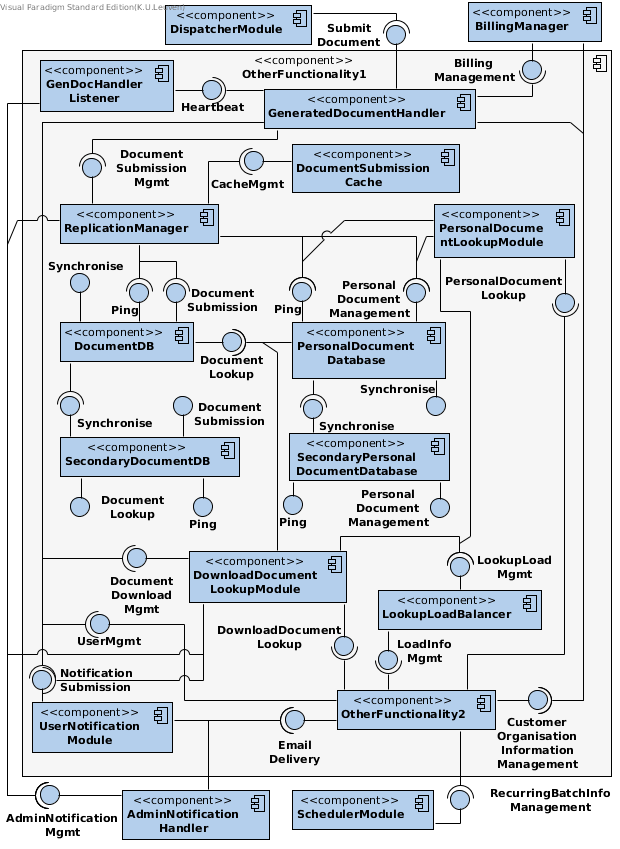
\includegraphics[width=0.8\textwidth]{comp_diag_2.png}
    %\missingfigure[figwidth=0.8\textwidth]{Component-and-connector diagram}
    \caption{Component-and-connector diagram of this decomposition.
        }\label{fig:it2-cc_main}
\end{figure}

\paragraph{Deployment}
Figure \ref{fig:it2-depl_main} shows the mapping of architectural components on physical nodes. Only the components introduced in this run and previously connected to the decomposed component \texttt{OtherFunctionality1} are shown as per the component-and-connector diagram. The \texttt{RawDataHandlingNode} and \texttt{PrimaryDispatcher} are the same nodes as in the first run. The \texttt{DocumentHandlerNode} contains the entry point for the delivery and storage system for documents, along with its heartbeat listener. The \texttt{DatabaseReplicationNode}, \texttt{DocumentDB}, \texttt{SecondaryDocumentDB}, \texttt{PersonalDocumentDatabase} and \texttt{SecondaryPersonalDocumentDatabase} are the database nodes along with their passive replication nodes. They are all seperate nodes so failure of one does not cause document loss. The \texttt{LookupNode} contains all components regarding document lookup. The \texttt{OtherFunctionalityNode} contains all other components not directly impacted by this run.

\begin{figure}[!htp]
    \centering
    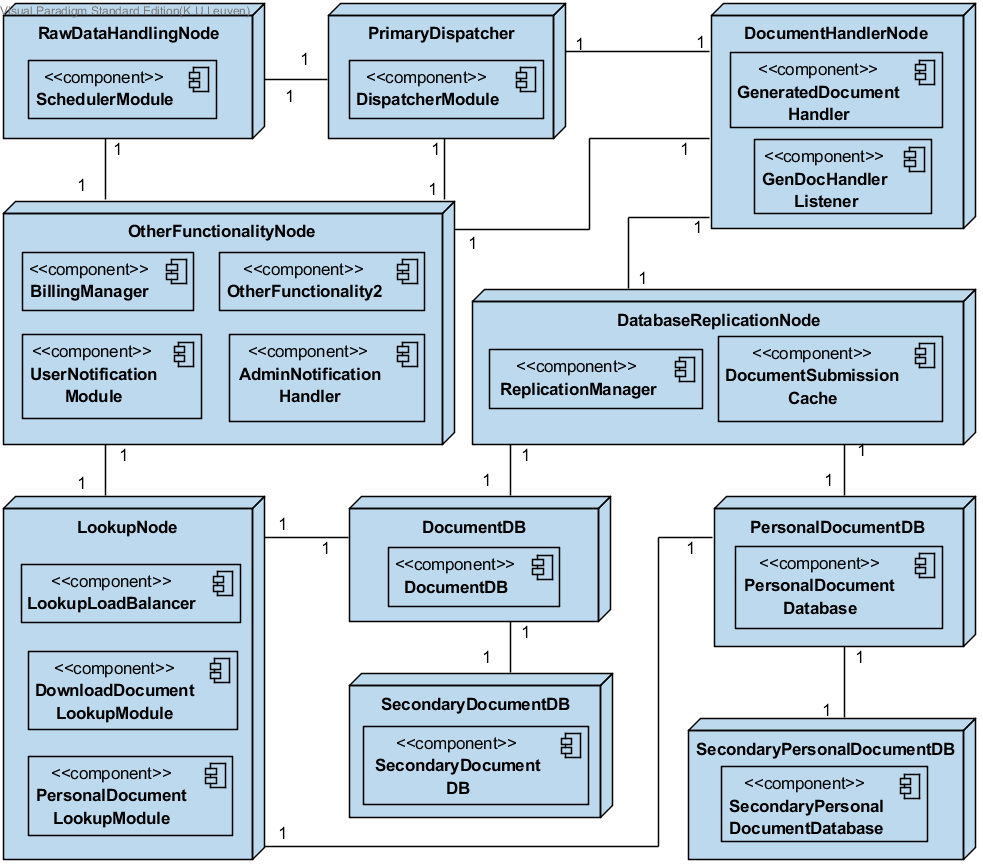
\includegraphics[width=0.8\textwidth]{depl_diag_2.png}
    %\missingfigure[figwidth=0.8\textwidth]{Deployment diagram}
    \caption{Deployment diagram of this decomposition.
        }\label{fig:it2-depl_main}
\end{figure}

\subsubsection{Interfaces for child modules}
\subsubsection*{DocumentDB}
\begin{itemize}
    \item DocumentSubmission
    \begin{itemize}
        \item \texttt{void submitDocument(DocumentData doc)}
        \begin{itemize}
            \item Effect: Writes the specified generated document into the database.
            \item Exceptions: None
        \end{itemize}

        \item \texttt{void removeDocument(DocumentDataID id)}
        \begin{itemize}
            \item Effect: Removes the document specified by id from the database. No effect if no such document exists.
            \item Exceptions: None
         \end{itemize}
    \end{itemize}

    \item DocumentLookup
    	\begin{itemize}
    		\item \texttt{DocumentData retrieveDocumentData(DocumentDataID id)} throws NoSuchDocumentException
    		\begin{itemize}
    			\item Effect: Retrieves the full document data matching the specified id.
    			\item Exceptions:
    			\begin{itemize}
    				\item NoSuchDocumentException: no document matching the specified id is present
    			\end{itemize}
    		\end{itemize}

    		\item \texttt{Document retrieveDocument(DocumentDataID id)} throws NoSuchDocumentException
    		\begin{itemize}
    			\item Effect: Retrieves the generated document without its raw data.
    			\item Exceptions:
    			\begin{itemize}
    				\item NoSuchDocumentException: no document matching the specified id is present
    			\end{itemize}
    		\end{itemize}

    		\item \texttt{RawDataEntry retrieveRawDataFromDocument(DocumentDataID id)} throws NoSuchDocumentException
    		\begin{itemize}
    			\item Effect: Retrieves the raw data of the specified document.
    			\item Exceptions:
    			\begin{itemize}
    				\item NoSuchDocumentException: no document matching the specified id is present
    			\end{itemize}
    		\end{itemize}

    		\item \texttt{List<DocumentData> queryDocumentData(DocumentQuery query)}
    		\begin{itemize}
    			\item Effect: Retrieves the full document data of all documents that satisfy the specified DocumentQuery.
    			\item Exceptions: None
    		\end{itemize}

    		\item \texttt{List<Document> queryDocuments(DocumentQuery query)}
    		\begin{itemize}
    			\item Effect: Retrieves all generated documents that satisfy the specified DocumentQuery, without their raw data.
    			\item Exceptions: None
    		\end{itemize}

    		\item \texttt{List<RawDataEntry> queryRawDataFromDocuments(DocumentQuery query)}
    		\begin{itemize}
    			\item Effect: Retrieves the raw data of the all documents that satisfy the specified DocumentQuery.
    			\item Exceptions: None
    		\end{itemize}
    	\end{itemize}


    \item Synchronise
    	\begin{itemize}
    		\item \texttt{void synchroniseState(List<DocumentDataUpdate> updates)}
    		\begin{itemize}
    			\item Effect: Carries out all updates contained within the specified list.
    			\item Exceptions: None
    		\end{itemize}
    	\end{itemize}

    \item Ping
    \begin{itemize}
    	\item \texttt{Echo ping()}
    	\begin{itemize}
    		\item Effect: Returns an Echo to reassure the caller that the callee is still available.
    		\item Exceptions: None
    	\end{itemize}
    \end{itemize}
\end{itemize}

\subsubsection*{PersonalDocumentDatabase}
\begin{itemize}
	\item PersonalDocumentManagement
	\begin{itemize}
		\item \texttt{void submitPersonalDocument(DocumentData doc, RegisteredRecipientID id)}
		\begin{itemize}
			\item Effect: Submits the specified document with the specified Registered Recipient to the \texttt{PersonalDocumentDatabase}.
			\item Exceptions: None
		\end{itemize}

		\item \texttt{void removePersonalDocument(DocumentDataID docID)}
		\begin{itemize}
			\item Effect: Removes the specified document identifier from the database. No effect if no such document exists.
			\item Exceptions: None
		\end{itemize}

		\item \texttt{void removePersonalDocumentAssociation(DocumentDataID docID)}
		\begin{itemize}
			\item Effect: Removes the association between the specified document with its recipient identifier. No effect if no such document exists.
			\item Exceptions: None
		\end{itemize}

		\item \texttt{DocumentData retrievePersonalDocumentData(DocumentDataID docID, RegisteredRecipientID id)} throws NoSuchDocumentException, RetrievalNotAllowedException
		\begin{itemize}
			\item Effect: Retrieves the full document data specified by the given document identifier.
			\item Exceptions:
			\begin{itemize}
				\item NoSuchDocumentException: The specified DocumentDataID is not present.
				\item RetrievalNotAllowedException: The specified document does not belong to the personal document store of the specified recipient.
			\end{itemize}
		\end{itemize}

		\item \texttt{Document retrievePersonalDocument(DocumentDataID docID, RegisteredRecipientID id)} throws NoSuchDocumentException, RetrievalNotAllowedException
		\begin{itemize}
			\item Effect: Retrieves the document specified by the given document identifier without its raw data.
			\item Exceptions:
			\begin{itemize}
				\item NoSuchDocumentException: The specified DocumentDataID is not present.
				\item RetrievalNotAllowedException: The specified document does not belong to the personal document store of the specified recipient.
			\end{itemize}
		\end{itemize}

		\item \texttt{RawDataEntry retrievePersonalDocumentRawData(DocumentDataID docID, RegisteredRecipientID id)} throws NoSuchDocumentException, RetrievalNotAllowedException
		\begin{itemize}
			\item Effect: Retrieves the raw data belonging to the document specified by the given document identifier.
			\item Exceptions:
			\begin{itemize}
				\item NoSuchDocumentException: The specified DocumentDataID is not present.
				\item RetrievalNotAllowedException: The specified document does not belong to the personal document store of the specified recipient.
			\end{itemize}
		\end{itemize}

		\item \texttt{List<DocumentData> queryPersonalDocumentData(DocumentQuery query)} throws RecipientIDNotIncludedException
		\begin{itemize}
			\item Effect: Retrieves the full document data of all documents matching the specified DocumentQuery.
			\item Exceptions:
			\begin{itemize}
				\item RecipientIDNotIncludedException: The DocumentQuery does not include the identifier of the recipient
			\end{itemize}
		\end{itemize}

		\item \texttt{List<Document> queryPersonalDocuments(DocumentQuery query)} throws RecipientIDNotIncludedException
		\begin{itemize}
			\item Effect: Retrieves all documents matching the specified DocumentQuery without their raw data.
			\item Exceptions:
			\begin{itemize}
				\item RecipientIDNotIncludedException: The DocumentQuery does not include the identifier of the recipient
			\end{itemize}
		\end{itemize}

		\item \texttt{List<RawDataEntry> queryPersonalDocumentRawData(DocumentQuery query)} throws RecipientIDNotIncludedException
		\begin{itemize}
			\item Effect: Retrieves the raw data of all documents matching the specified DocumentQuery.
			\item Exceptions:
			\begin{itemize}
				\item RecipientIDNotIncludedException: The DocumentQuery does not include the identifier of the recipient
			\end{itemize}
		\end{itemize}
	\end{itemize}

	\item Synchronise
	\begin{itemize}
		\item \texttt{void synchroniseState(List<PersonalDocumentDataUpdate> updates)}
		\begin{itemize}
			\item Effect: Carries out all updates contained within the specified list.
			\item Exceptions: None
		\end{itemize}
	\end{itemize}

	\item Ping
	\begin{itemize}
		\item \texttt{Echo ping()}
		\begin{itemize}
			\item Effect: Returns an Echo to reassure the caller that the callee is still available.
			\item Exceptions: None
		\end{itemize}
	\end{itemize}
\end{itemize}

\subsubsection*{DocumentSubmissionCache}
\begin{itemize}
	\item CacheManagement
	\begin{itemize}
		\item \texttt{void submitDocumentUpdate(DocumentDataUpdate update)}
		\begin{itemize}
			\item Effect: Records the specified update in the cache.
			\item Exceptions: None
		\end{itemize}

		\item \texttt{void submitPersonalDocumentUpdate(PersonalDocumentDataUpdate update)}
		\begin{itemize}
			\item Effect: Records the specified update in the cache.
			\item Exceptions: None
		\end{itemize}

		\item \texttt{List<DocumentDataUpdate> flushDocumentDataUpdates()}
		\begin{itemize}
			\item Effect: Retrieves all stored document data updates and removes these.
			\item Exceptions: None
		\end{itemize}

		\item \texttt{List<PersonalDocumentDataUpdate> flushPersonalDocumentDataUpdates()}
		\begin{itemize}
			\item Effect: Retrieves all stored personal document data updates and removes these.
			\item Exceptions: None
		\end{itemize}

		\item \texttt{void removeDocumentUpdate(DocumentDataID id)}
		\begin{itemize}
			\item Effect: Removes any updates pertaining to the specified document from the cache.
			\item Exceptions: None
		\end{itemize}

		\item \texttt{void removePersonalDocumentUpdate(DocumentDataID docID)}
		\begin{itemize}
			\item Effect: Removes any personal document database updates pertaining to the specified document from the cache.
			\item Exceptions: None
		\end{itemize}
	\end{itemize}
\end{itemize}

\subsubsection*{ReplicationManager}
\begin{itemize}
	\item DocumentSubmissionManagement
	\begin{itemize}
		\item \texttt{void submitDocument(DocumentData doc, boolean addToPersonalDB)}
		\begin{itemize}
			\item Effect: Writes the specified generated document into the document database. If addToPersonalDB is true, then the document, together with the recipient's identifier is written to the personal document database
			\item Exceptions: None
		\end{itemize}

		\item \texttt{void addDocumentsToPersonalDocumentStore(RegisteredRecipientID id)}
		\begin{itemize}
			\item Effect: Looks up all document identifiers belonging to the specified recipient in the \texttt{DocumentDB}, and writes those pairs to the personal document database
			\item Exceptions: None
		\end{itemize}

		\item \texttt{void removeDocumentsFromPersonalDocumentStore(RegisteredRecipientID id)}
		\begin{itemize}
			\item Effect: Looks up all associations between document identifiers and the specified recipient in the personal document database and removes them
			\item Exceptions: None
		\end{itemize}
	\end{itemize}

	\item ReplicationConfirmation
	\begin{itemize}
		\item \texttt{void confirmDocumentUpdateSuccess(DocumentDataID id)}
		\begin{itemize}
			\item Effect: Confirms that all updates concerning the specified documents in the document database were successful.
			\item Exceptions: None
		\end{itemize}

		\item \texttt{void confirmPersonalDocumentUpdateSuccess(DocumentDataID id)}
		\begin{itemize}
			\item Effect: Confirms that all updates concerning the specified documents in the personal document database were successful.
			\item Exceptions: None
		\end{itemize}
	\end{itemize}
\end{itemize}

\subsubsection*{GeneratedDocumentHandler}
\begin{itemize}
    \item SubmitDocument
    This is the same interface as presented by \texttt{OtherFunctionality1} after the first run.
\end{itemize}

\subsubsection*{GenDocHandlerListener}
\begin{itemize}
    \item Heartbeat
    \begin{itemize}
        \item \texttt{void supplyHeartbeat()}
        \begin{itemize}
            \item Effect: Records a heartbeat from the supervised component.
            \item Exceptions: None
        \end{itemize}
    \end{itemize}
\end{itemize}

\subsubsection*{PersonalDocumentLookupModule}
\begin{itemize}
    \item PersonalDocumentLookup
    \begin{itemize}
        \item \texttt{Document retrievePersonalDocument(DocumentDataID docID, RegisteredRecipientID id)} throws NoSuchDocumentException, RetrievalNotAllowedException
        \begin{itemize}
            \item Effect: Retrieves the document specified by the given document identifier without its raw data.
            \item Exceptions:
            \begin{itemize}
                \item NoSuchDocumentException: The specified DocumentDataID is not present.
                \item RetrievalNotAllowedException: The specified document does not belong to the personal document store of the specified recipient.
            \end{itemize}
        \end{itemize}

        \item \texttt{List<Document> queryPersonalDocuments(DocumentQuery query)} throws RecipientIDNotIncludedException
        \begin{itemize}
            \item Effect: Retrieves all documents matching the specified DocumentQuery without their raw data.
            \item Exceptions:
            \begin{itemize}
                \item RecipientIDNotIncludedException: The DocumentQuery does not include the identifier of the recipient
            \end{itemize}
        \end{itemize}

        \item \texttt{List<Document> retrieveAllPersonalDocuments(RegisteredRecipientID id)} throws NoSuchRegisteredRecipientException
        \begin{itemize}
            \item Effect: Retrieves all documents of specified Registered Recipient's personal document store.
            \item Exceptions:
            \begin{itemize}
                \item NoSuchRegisteredRecipientException: The specified RegisteredRecipientID is not present in the system.
            \end{itemize}
        \end{itemize}
    \end{itemize}
\end{itemize}

\subsubsection*{DownloadDocumentLookupModule}
\begin{itemize}
    \item DocumentDownloadMgmt
    \begin{itemize}
        \item \texttt{void RecordDocumentDownloadDeadline(UnregisteredRecipientInfo recipientInfo, DocumentDataID docID, Time deadline)}
        \begin{itemize}
            \item Effect: Records the deadline for given Unregistered Recipient to download given document.
            \item Exceptions: None
        \end{itemize}
    \end{itemize}

    \item DownloadDocumentLookup
    \begin{itemize}
        \item \texttt{Document downloadDocument(DocumentDownloadToken token)} throws NoSuchDocumentException, RetrievalNotAllowedException
        \begin{itemize}
            \item Effect: Retrieves the document specified by the given token. Also records the fact that the document has been downloaded at least once.
            \item Exceptions:
            \begin{itemize}
                \item NoSuchDocumentException: The document specified in the token is not present.
                \item RetrievalNotAllowedException: The information in the token is not consistent with the download records in the module.
            \end{itemize}
        \end{itemize}
    \end{itemize}
\end{itemize}

\subsubsection*{LookupLoadBalancer}
\begin{itemize}
    \item LookupLoadMgmt
    \begin{itemize}
        \item \texttt{boolean requestLookupPermission(LookupSpecification specs)}
        \begin{itemize}
            \item Effect: Requests permission to perform the lookup as detailed by the Specification. This method returns a simple boolean whether or not the requesting module has permission to perform the actual lookup.
            \item Exceptions: None
        \end{itemize}

        \item \texttt{void submitLookupDelay(LookupSpecification specs, Time delay)}
        \begin{itemize}
            \item Effect: Records internally the source of the lookup, the amount of looked up documents and the encountered delay while looking up documents. These are recorded to calculate the current load of the databases, and to prepare answers for future lookup requests.
        \end{itemize}
    \end{itemize}

    \item LoadInfoMgmt
    \begin{itemize}
        \item \texttt{void submitCurrentDatabasesSpecs(List<DatabaseSpecification> specs)} throws InconsistentDatabaseSetupException
        \begin{itemize}
            \item Effect: The \texttt{Loadbalancer} assumes the received list details the (new) full set of databases available to the system, and sets these as a reference for lookup load calculation.
            \item Exceptions:
            \begin{itemize}
                \item InconsistentDatabaseSetupException: When the supplied list of \texttt{Databases} is not consistent with the amount or type of \texttt{Databases} expected by the \texttt{LoadBalancer}.
            \end{itemize}
        \end{itemize}
    \end{itemize}
\end{itemize}

\subsubsection*{RecipientNotificationModule}
\begin{itemize}
    \item NotificationSubmission
    \begin{itemize}
        \item \texttt{void notifyUnregisteredRecipient(UnregisteredRecipientInfo info, NotificationContents contents)}
        \begin{itemize}
            \item Effect: Composes an e-mail to given recipient with given contents, and submits it for delivery.
            \item Exceptions: None
        \end{itemize}

        \item \texttt{void notifyRegisteredRecipient(RegisteredRecipientID id, NotificationContents contents)} throws NoSuchRegisteredRecipientException
        \begin{itemize}
            \item Effect: Composes an e-mail to given recipient with given contents, and submits it for delivery.
            \item Exceptions:
            \begin{itemize}
                \item NoSuchRegisteredRecipientException: The specified RegisteredRecipientID is not present in the system.
            \end{itemize}
        \end{itemize}
    \end{itemize}
\end{itemize}

\subsubsection*{OtherFunctionality2}
\begin{itemize}
    \item EmailDelivery
    \begin{itemize}
        \item \texttt{void submitEmailWithDestination(String emailAddress, HTMLDocument mail)}
        \begin{itemize}
            \item Effect: Submit an email document for delivery to supplied e-mail address.
            \item Exceptions: None
        \end{itemize}

        \item \texttt{void submitEmailWithRegisteredRecipientID(RegisteredRecipientID id, HTMLDocument mail)} throws NoSuchRegisteredRecipientException
        \begin{itemize}
            \item Effect: Submit an email document for delivery to Registered Recipient with given id.
            \item Exceptions:
            \begin{itemize}
                \item NoSuchRegisteredRecipientException: The specified RegisteredRecipientID is not present in the system.
            \end{itemize}
        \end{itemize}
    \end{itemize}

    \item RecipientMgmt
    \begin{itemize}
        \item \texttt{boolean isRegisteredRecipient(String emailAddress)}
        \begin{itemize}
            \item Effect: Check whether or not the recipient with given e-mail address is a Registered Recipient.
            \item Exceptions: None
        \end{itemize}

        \item \texttt{RegisteredRecipientID lookupRegisterRecipientID(String emailAddress)} throws NoSuchRegisteredRecipientException
        \begin{itemize}
            \item Effect: Lookup the ID of the Registered Recipient with given e-mail address.
            \item Exceptions:
            \begin{itemize}
                \item NoSuchRegisteredRecipientException: When the given e-mail address does not belong to a Registered Recipient.
            \end{itemize}
        \end{itemize}
    \end{itemize}

    \item CustomerOrganisationInfoManagement
    This is the same interface as presented by \texttt{OtherFunctionality1} after the first run, along with following additions:
    \begin{itemize}
        \item \texttt{void requestOrganisationBilling(BillingRequest request)} throws IncorrectlySignedException
        \begin{itemize}
            \item Effect: Submits a request for billing a Customer Organisation for planned and unplanned expenses in the system.
            \item Exceptions:
            \begin{itemize}
                \item IncorrectlySignedException: When the request was not signed by a trusted billing component.
            \end{itemize}
        \end{itemize}

        \item \texttt{RecurringBatchDetails getOrganisationRecurringBatchDetails(OrganisationID id)}
        \begin{itemize}
            \item Effect: Request the RecurringBatchDetails for Customer Organisation with given ID.
        \end{itemize}
    \end{itemize}
\end{itemize}

\subsubsection{Data type definitions}
Describe per complex data type used in the interfaces what it represents.

\paragraph{DocumentQuery} Represents an executable query on both the document database and the personal document database. A non-exhaustive list of elements are the name of the sender, a date range, document type or identifier of a registered recipient

\paragraph{DocumentDataUpdate} Contains a DocumentData instance and an indication whether this is a write or a removal.

\paragraph{PersonalDocumentDataUpdate} Contains an association between a DocumentDataID and a RegisteredRecipientID and an indication whether this is a write or a removal

\paragraph{RegisteredRecipientID} Corresponds with a single registered recipient. Currently, this identifier is envisioned as the recipient's e-mail address.

\paragraph{UnregisteredRecipientInfo} Information to identify and if necessary contact an Unregistered Recipient.

\paragraph{DocumentDownloadToken} A token generated for the Unregistered recipient, containing their UnregisteredRecipientInfo and DocumentDataID. This token can be used with the system to download a document, as long as the deadline for the download is not reached.

\paragraph{LookupSpecification} A specification of a certain lookup action, detailing the target database for lookup, the source lookup module and the amount and estimated size of all documents in the lookup.

\paragraph{DatabaseSpecification} A specification of a database in the system, containing an identifier and the resources it has for lookup and storage.

\paragraph{NotificationContents} Contents for a message to deliver to a message recipient.

\paragraph{BillingRequest} Details of billing to a given Customer Organisation, containing among other information at least the amount the Organisation should be billed for, and details of how the amount was calculated. This request should be signed by a trusted billing component, here the \texttt{BillingManager}.

\paragraph{RecurringBatchDetails} Details for a Customer Organisation about the recurring batches as agreed with the eDocs company in their SLA.

\subsubsection{Verify and refine}
This section describes per component which (parts of) the remaining requirements it is responsible for. If requirements are split, a letter is added to its name (e.g. Av1a) to indicate that the component will only satisfy a part of the original requirement. If requirements are split, it will also be indicated what part of the original requirement each new requirement contains. If new derived requirements are introduced they will receive a new identifier and are marked as a new requirement.

\paragraph{OtherFunctionality2}
\begin{itemize}
    \item \emph{UC1}: Log in
    \item \emph{UC2}: Log out
    \item \emph{UC6}: Deliver document via e-mail
    \item \emph{UC8}: Deliver document via postal mail
    \item \emph{UC9}: Deliver document via Zoomit
    \item \emph{UC10}: Confirm document delivery (Zoomit)
    \item \emph{UC15a}: Download document via document link\\
    Issuing the request for download of the specified document
    \item \emph{UC16}: Register to personal document store
    \item \emph{UC17}: Unregister from personal document store
    \item \emph{UC18}: Register customer organization
    \item \emph{UC19}: Unregister customer organization
    \item \emph{UC20}: Update document template
    \item \emph{UC21a}: Consult status of all document processing jobs\\
    Handling the (visual) interfacing with the user. Determining the finished jobs.
    \item \emph{UC22a}: Notify customer administrator\\
    Notifying the customer administrator of delivery failure
    \item \emph{Av3}: Zoomit failure
    \item \emph{P3b}: Status overview for customer administrators\\
    Handling the (visual) interfacing with the user
    \item \emph{M1a}: New type of document: bank statements\\
    The delivery and template handling for the new document
    \item \emph{M2}: Multiple print \& postal services
    \item \emph{M3}: Dynamic selection of the cheapest of print \& postal services
\end{itemize}

\paragraph{SubmissionSubsystem}
\begin{itemize}
	\item \emph{UC3}: Initiate document processing
	\item \emph{M1b}: New type of document: bank statements\\
	Being able to receive and verify the integrity of Raw Data for the new type of document.
\end{itemize}

\paragraph{RawDataPool}
\begin{itemize}
	\item \emph{UC21b}: Consult status of all document processing jobs\\
	Determining the unfinished and currently processing jobs.
	\item \emph{P3b}: Status overview for customer administrators\\
	Calculating and delivering information about all unfinished and currently processing jobs for a certain \texttt{Customer Organisation} in a timely fashion.
\end{itemize}

\paragraph{DocumentGenerationProcess}
\begin{itemize}
	\item \emph{M1c}: New type of document: bank statements\\
	Being able to generate documents of the new type with the accompanying new template.
\end{itemize}

\subsection{Decomposition 3: OtherFunctionality2 (UC1, UC2, UC16, UC17, UC18, UC19)}
\subsubsection{Module to decompose}
In this run we decompose \texttt{OtherFunctionality2}. This component is an aggregate of leftover behaviour in the previous run.

\subsubsection{Selected architectural drivers}

The related functional drivers are:

\begin{itemize}
    \item \emph{UC1}: Log in
    \item \emph{UC2}: Log out
    \item \emph{UC16}: Register to personal document store
    \item \emph{UC17}: Unregister from personal document store
    \item \emph{UC18}: Register customer organization
    \item \emph{UC19}: Unregister customer organization
\end{itemize}

\paragraph{Rationale}
This set of use-cases is very coherent and complete as a group. Most are high-priority or medium-priority use-cases. N quality requirement matches any of the use-cases so none were selected. This is also supported by the fact that all but one remaining quality requirements are low-priority, the other one being medium-priority.

\subsubsection{Architectural design}
\paragraph{Topic}
Discussion of the solution selected for (a part of) one of the architectural
drivers.

\subsubsection*{Alternatives considered}
\paragraph{Alternatives for solution}
A discussion of the alternative solutions and why that were not selected.

\subsubsection{Instantiation and allocation of functionality}
\paragraph{Decomposition}
Main aspects of the resulting decomposition.

\subparagraph{ModuleB}
Per introduced component a paragraph describing its responsibilities.

\subparagraph{ModuleC}
Per introduced component a paragraph describing its responsibilities.

\begin{figure}[!htp]
    \centering
    %\includegraphics[width=0.8\textwidth]{}
    \missingfigure[figwidth=0.8\textwidth]{Component-and-connector diagram}
    \caption{Component-and-connector diagram of this decomposition.
        }\label{fig:it1-cc_main}
\end{figure}

\paragraph{Behaviour}
If needed and explanation of the behaviour of certain aspects of the design so
far.

\begin{figure}[!htp]
    \centering
    %\includegraphics[width=0.8\textwidth]{}
    \missingfigure[figwidth=0.8\textwidth]{Sequence diagram}
    \caption{Sequence diagram illustrating a key behavioural aspect.
        }\label{fig:it1-seq_aspect1}
\end{figure}

\paragraph{Deployment}
Rationale of the allocation of components to physical nodes.

\begin{figure}[!htp]
    \centering
    %\includegraphics[width=0.8\textwidth]{}
    \missingfigure[figwidth=0.8\textwidth]{Deployment diagram}
    \caption{Deployment diagram of this decomposition.
        }\label{fig:it1-depl_main}
\end{figure}

\subsubsection{Interfaces for child modules}
\subsubsection*{ModuleB}
\begin{itemize}
    \item InterfaceA
    \begin{itemize}
        \item \texttt{returnType operation1(ParamType param1)} throws TypeOfException
        \begin{itemize}
            \item Effect: Describe the effect of calling this operation.
            \item Exceptions: 
            \begin{itemize}
                \item TypeOfException: Describe when this exception is thrown.
            \end{itemize}
        \end{itemize}

        \item \texttt{returnType operation2()}
        \begin{itemize}
            \item Effect: Describe the effect of calling this operation.
            \item Exceptions: None
         \end{itemize}
    \end{itemize}
\end{itemize}

\subsubsection{Data type definitions}
Describe per complex data type used in the interfaces what it represents.

\paragraph{returnType} This data element represents X.

\paragraph{ParamType} This data element represents Y.

\subsubsection{Verify and refine}
This section describes per component which (parts of) the remaining
requirements it is responsible for.

\paragraph{ModuleB}
\begin{itemize}
    \item \emph{Z1}: name
    \item \emph{UCd}: name
\end{itemize}

\paragraph{ModuleC}
\begin{itemize}
    \item \emph{UCba}: name\\Description which part of the original use case is
        the responsibility of this component.
\end{itemize}

\section{Resulting partial architecture}\label{sec:architecture}
This section provides an over of the architecture constructed through ADD\@.

\subsection{Context diagram}
This subsection discusses the context diagram.

\begin{figure}[!htp]
    \centering
    %\includegraphics[width=0.8\textwidth]{}
    \missingfigure[figwidth=0.8\textwidth]{Context diagram for component-and-
        connector view.}
    \caption{Context diagram for the component-and-connector view.
        }\label{fig:cc_context}
\end{figure}

\subsection{Component-and-connector view}
A short discussion of the component-and-connector view with the key
decompositions if any.

\begin{figure}[!htp]
    \centering
    %\includegraphics[width=0.8\textwidth]{}
    \missingfigure[figwidth=0.8\textwidth]{Component-and-connector diagram}
    \caption{Primary diagram for the component-and-connector view.
        }\label{fig:cc_main}
\end{figure}

\begin{figure}[!htp]
    \centering
    %\includegraphics[width=0.8\textwidth]{}
    \missingfigure[figwidth=0.8\textwidth]{Key decomposition}
    \caption{Decomposition of a component shown in Figure~\ref{fig:cc_main}
        }\label{fig:decomp_decomp1}
\end{figure}

\subsection{Deployment view}
A short discussion of the allocation of components to physical nodes based on a
context diagram and a deployment diagram.

\begin{figure}[!htp]
    \centering
    %\includegraphics[width=0.8\textwidth]{}
    \missingfigure[figwidth=0.8\textwidth]{Context diagram for the allocation
        view.}
    \caption{Context diagram for the allocation view.}\label{fig:depl_context}
\end{figure}

\begin{figure}[!htp]
    \centering
    %\includegraphics[width=0.8\textwidth]{}
    \missingfigure[figwidth=0.8\textwidth]{Deployment diagram}
    \caption{Primary diagram for the allocation view.}\label{fig:depl_main}
\end{figure}

\end{document}
